\chapter{DATASET AND PREPROCESSING}
\graphicspath{{Chapter2/}}

\section{Dataset}

Many gait datasets are available like CASIA, OU-ISIR. For our project we have used CASIA-B Gait silhouette images as input.

\subsection{CASIA-B}
Dataset B[1] is a large multi view gait database. It is Created in January 2005. There are 124 subjects (93 males, 31 females). Gait data was captured from 11 views. Three variations, namely view angle, clothing and carrying condition changes, are separately considered. Human silhouettes extracted from video files are also available.\cite{shiqi2006}

\section{Preprocessing}

\subsection{Gait Energy Image (GEI)}

After categorizing silhouette images of a walk into 11 groups, the silhouette images in the same group (except the rejected group) are combined to form 10 GEIs. For each GEI, its value at position (x, y) is defined by;

$$ GEI(x, y) = \sum_{t=1}^{n} I_t(x, y) $$

where N is the number of silhouette images in a group, It (x, y) is the value at position (x, y) of the tth image in the group.
\begin{figure}[ht]
    \centering
    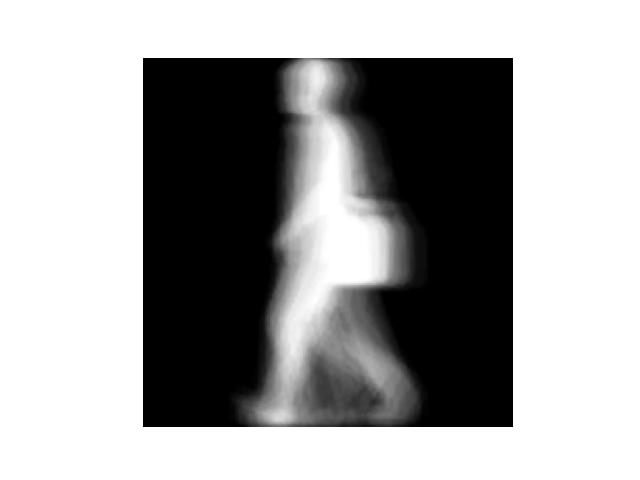
\includegraphics[scale=0.6]{data/gei.png}
    \caption{Gait Energy Image}
    \label{fig:gei}
\end{figure}

\subsection{Multi channel GEI}
Multi-channel GEI involves extracting features from the multi-dimensional gait data. This often involves calculating the covariance matrices of the data from each sensor/channel and then finding the eigenvectors and eigenvalues of these matrices. These eigenvectors represent the principal components of variation in the gait data, while the eigenvalues indicate the significance of each component.\cite{kitchat2019}

\begin{figure}[ht]
    \centering
    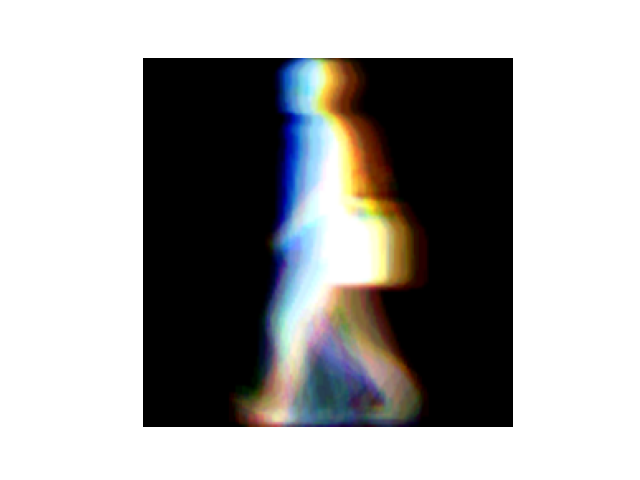
\includegraphics[scale=0.6]{data-3/gei3.png}
    \caption{3-channel GEI}
    \label{fig:gei-3}
\end{figure}
